\documentclass[12pt]{article}

\usepackage[margin=1in]{geometry}
\usepackage{fancyhdr}
\pagestyle{fancy}
\usepackage{amsmath}
\usepackage{amssymb}

% limit to particular location
\usepackage{float}

% graphics
\usepackage{graphicx}
% for subfigures
\usepackage{subcaption}

% better ref links
\usepackage{hyperref}

% footnote in footer
\newcommand{\fancyfootnotetext}[2]{%
  \fancypagestyle{dingens}{%
    \fancyfoot[LO,RE]{\parbox{7cm}{\footnotemark[#1]\footnotesize #2}}%
  }%
  \thispagestyle{dingens}%
}

\lhead{HW2}
\chead{Digital Image Processing}
\rhead{B03902036}


\begin{document}


\section*{Problem 1}
\subsection*{First-order edge detection}
\paragraph*{Robert filter} calculates diagonal edge gradients (\autoref{eq:robert_op}), susceptible to fluctuations and provides no information about edge orientation.

\begin{equation}
\label{eq:robert_op}
\begin{cases}
	G_x = \begin{bmatrix}
		1 & 0 \\ 0 & -1 
	\end{bmatrix} \ast I \\
	G_y = \begin{bmatrix}
		0 & 1 \\ -1 & 0
	\end{bmatrix} \ast I
\end{cases}
\end{equation}

\noindent
Gradient map is composed of
\begin{equation}
\label{eq:gx_gy_gxy}
	\nabla I(x, y) = G(x, y) = \sqrt{G_x^2 + G_y^2}
\end{equation}
and the edge map is determined by
\begin{equation}
\label{eq:edge_map}
E = 
\begin{cases}
	1, 2 \text{ S.D.}(\sim 5\%) \\
	0, \text{otherwise}
\end{cases}
\end{equation}

\begin{figure}[H]
    \centering
    \begin{subfigure}[t]{0.5\textwidth}
        \centering
        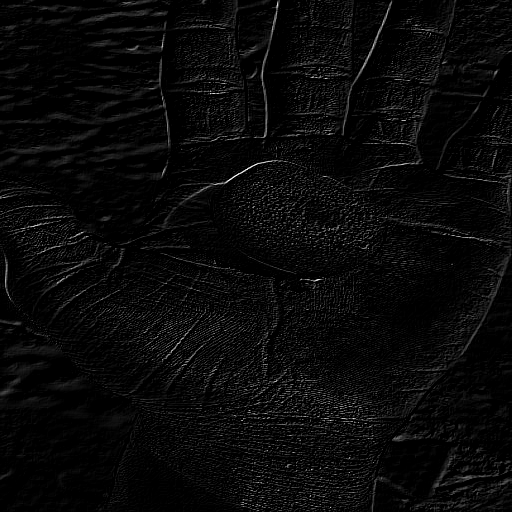
\includegraphics[height=2.5in]{images/robert_x}
        \caption{$I_x$}
    \end{subfigure}%
    ~ 
    \begin{subfigure}[t]{0.5\textwidth}
        \centering
        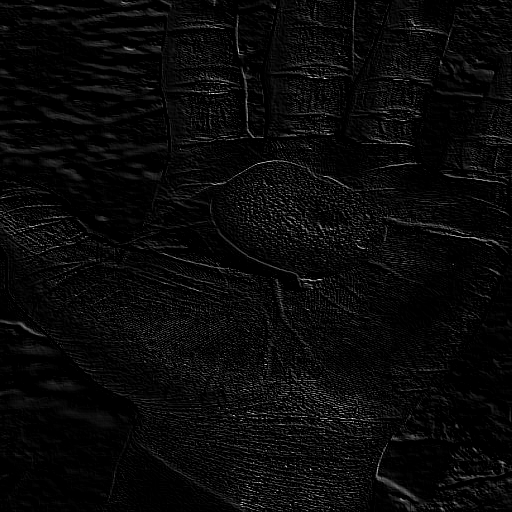
\includegraphics[height=2.5in]{images/robert_y}
        \caption{$I_y$}
    \end{subfigure}
    ~
    \vskip\baselineskip
    \begin{subfigure}[t]{0.5\textwidth}
        \centering
        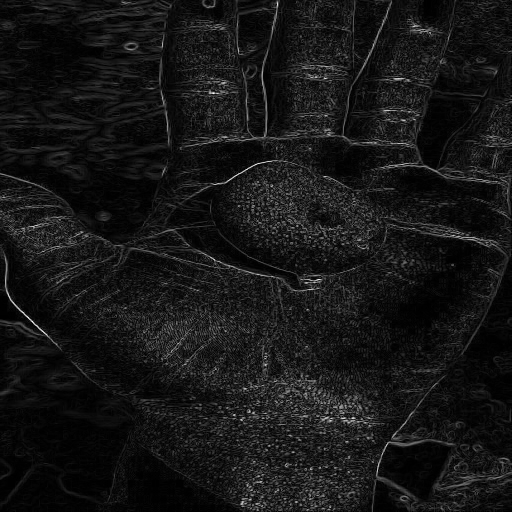
\includegraphics[height=2.5in]{images/robert_xy}
        \caption{$I_{xy}$}
    \end{subfigure}%
    ~
    \begin{subfigure}[t]{0.5\textwidth}
        \centering
        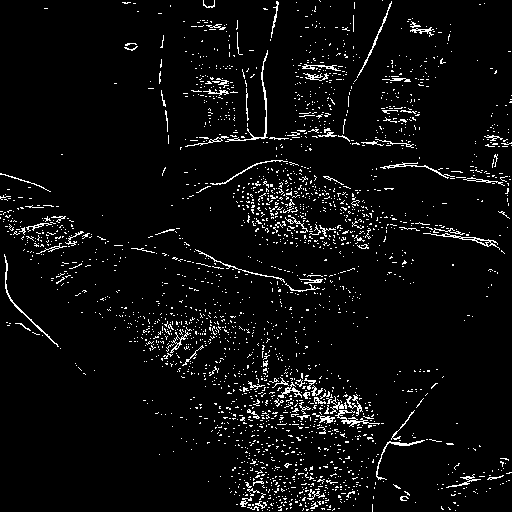
\includegraphics[height=2.5in]{images/robert_edge}
        \caption{Edge map}
    \end{subfigure}
    \caption{Robert operator}
\end{figure}

\paragraph*{Prewitt filter} is a discrete differentiation operator, which behaves similar to the Sobel operator by computing the gradient for the image intensity function as well.
It makes use of the maximum directional gradient. Though it is easy to implement, it is very sensitive to noise as well.

\begin{equation}
\label{eq:robert_op}
\begin{cases}
	G_x = \begin{bmatrix}
		-1 & 0 & 1 \\ -1 & 0 & 1 \\ -1 & 0 & 1 
	\end{bmatrix} \ast I\\
	G_y = \begin{bmatrix}
		-1 & -1 & -1 \\ 0 & 0 & 0 \\ 1 & 1 & 1
	\end{bmatrix} \ast I
\end{cases}
\end{equation}
The final gradient result calculates through \autoref{eq:gx_gy_gxy} and \autoref{eq:edge_map} as well.

\begin{figure}[H]
    \centering
    \begin{subfigure}[t]{0.5\textwidth}
        \centering
        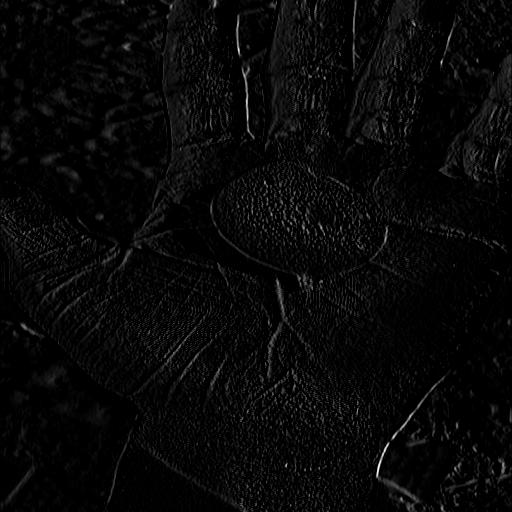
\includegraphics[height=2.5in]{images/prewitt_x}
        \caption{$I_x$}
    \end{subfigure}%
    ~ 
    \begin{subfigure}[t]{0.5\textwidth}
        \centering
        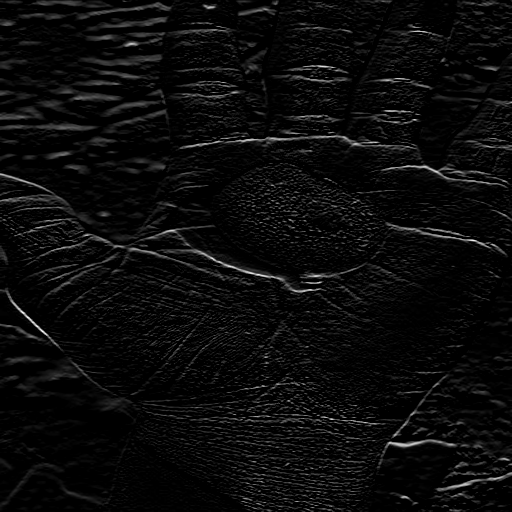
\includegraphics[height=2.5in]{images/prewitt_y}
        \caption{$I_y$}
    \end{subfigure}
    ~
    \vskip\baselineskip
    \begin{subfigure}[t]{0.5\textwidth}
        \centering
        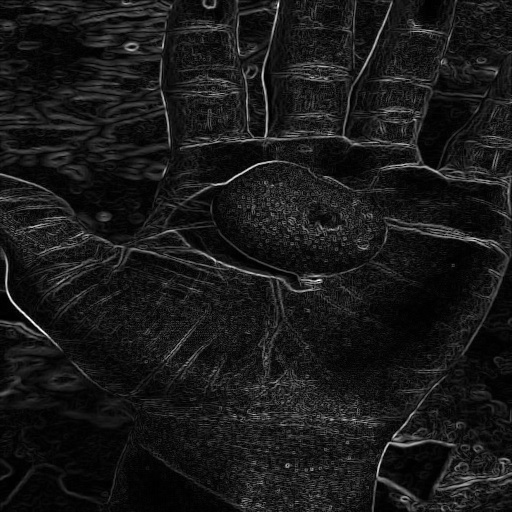
\includegraphics[height=2.5in]{images/prewitt_xy}
        \caption{$I_{xy}$}
    \end{subfigure}%
    ~
    \begin{subfigure}[t]{0.5\textwidth}
        \centering
        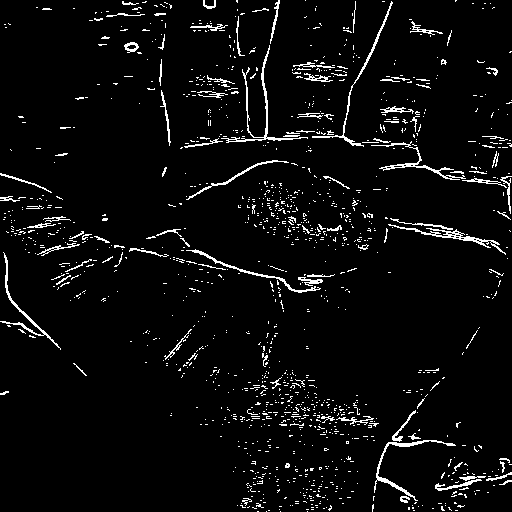
\includegraphics[height=2.5in]{images/prewitt_edge}
        \caption{Edge map}
    \end{subfigure}
    \caption{Prewitt operator}
\end{figure}

Noted that since Prewitt kernel can be decomposed, $G_x$ can be written as 
\begin{equation}
	G_x = \begin{bmatrix}
		-1 & 0 & 1 \\ -1 & 0 & 1 \\ -1 & 0 & 1 
	\end{bmatrix} \ast I
	= \begin{bmatrix}
		1 \\ 1 \\ 1 
	\end{bmatrix} \begin{bmatrix}
 		-1 & 0 & 1	
	\end{bmatrix}
	\ast I
\end{equation}
which essentially means that it computes the gradient with smoothing, since it can be decomposed as the products of an averaging and a differential kernel.

\paragraph*{Sobel filter} detects edges where the gradient magnitude is high. 
This makes the Sobel edge detector more sensitive to diagonal edge than horizontal (\autoref{fig:sobel_x}) and vertical edges (\autoref{fig:sobel_y}). 
Both Sobel filter and Prewitt filter are very effective at providing good edge maps.

\begin{equation}
\begin{cases}
	G_x = \begin{bmatrix}
		1 & 0 & -1 \\ 2 & 0 & -2 \\ 1 & 0 & -1 
	\end{bmatrix} \ast I \\
	G_y = \begin{bmatrix}
		1 & 2 & 1 \\ 0 & 0 & 0 \\ -1 & -2 & -1
	\end{bmatrix} \ast I
\end{cases}
\end{equation}

\noindent
The final gradient result calculates through \autoref{eq:gx_gy_gxy} and \autoref{eq:edge_map} as well.


\begin{figure}[H]
    \centering
    \begin{subfigure}[t]{0.5\textwidth}
        \centering
        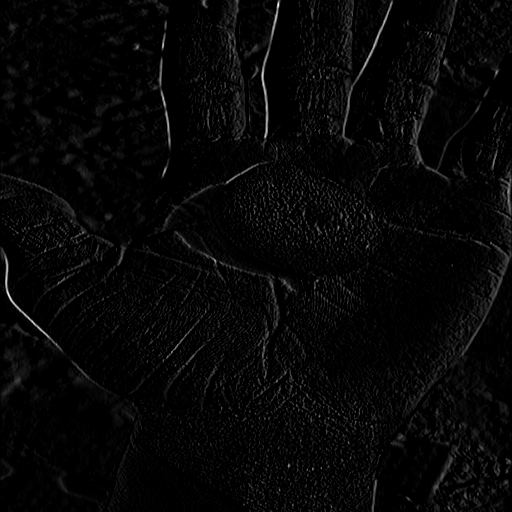
\includegraphics[height=2.5in]{images/sobel_x}
        \caption{$I_x$}
        \label{fig:sobel_x}
    \end{subfigure}%
    ~ 
    \begin{subfigure}[t]{0.5\textwidth}
        \centering
        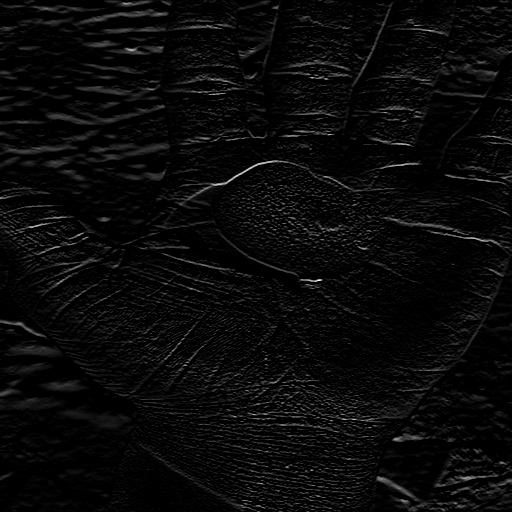
\includegraphics[height=2.5in]{images/sobel_y}
        \caption{$I_y$}
        \label{fig:sobel_y}
    \end{subfigure}
    ~
    \vskip\baselineskip
    \begin{subfigure}[t]{0.5\textwidth}
        \centering
        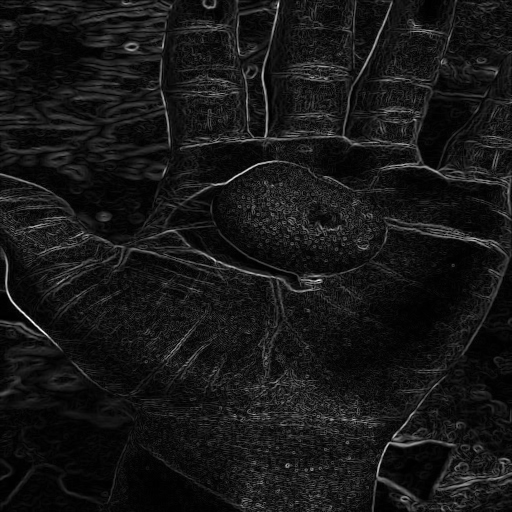
\includegraphics[height=2.5in]{images/sobel_xy}
        \caption{$I_{xy}$}
    \end{subfigure}%
    ~
    \begin{subfigure}[t]{0.5\textwidth}
        \centering
        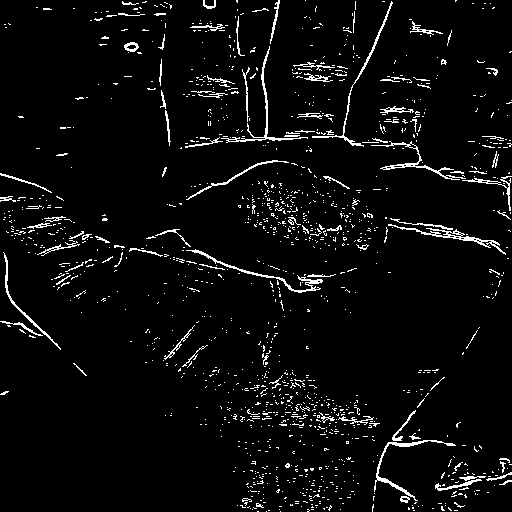
\includegraphics[height=2.5in]{images/sobel_edge}
        \caption{Edge map}
    \end{subfigure}
    \caption{Sobel operator}
\end{figure}

\subsection*{Second-order edge detection}
\paragraph*{Laplacian of Gaussian}
Laplacian filters are derivative filters used to find areas of rapid changing edges in images.

\begin{equation}
	\nabla^2 f(x, y) = \frac{\partial^2 f(x, y)}{\partial x^2} + \frac{\partial^2 f(x, y)}{\partial y^2}
\end{equation}

Since derivative filters are very sensitive to noise, it is common to smooth the image using a Gaussian filter before applying the Laplacian.

A possible approximation for the effect of the Laplacian is 
\begin{equation}
	K_L = \begin{bmatrix}
		0 & 1 & 0 \\ 1 & -4 & 1 \\ 0 & 1 & 0
	\end{bmatrix}
\end{equation}
One can reverse the sign of the elements of this negative Laplacian, but it does not affect the outcome.

To include a smoothing Gaussian lowpass filter, combine the Laplacian and Gaussian functions to obtain the result.
\begin{equation}
	K_{LoG} = -\frac{1}{\pi \sigma^4} \lbrack 1-\frac{x^2+y^2}{2 \sigma^2} \rbrack e^{-\frac{x^2 + y^2}{2 \sigma^2}}
\end{equation}
To utilize functions from previous homework, the calculation is still split instead of using a single kernel.

\begin{figure}[H]
    \centering
    \begin{subfigure}[t]{0.5\textwidth}
        \centering
        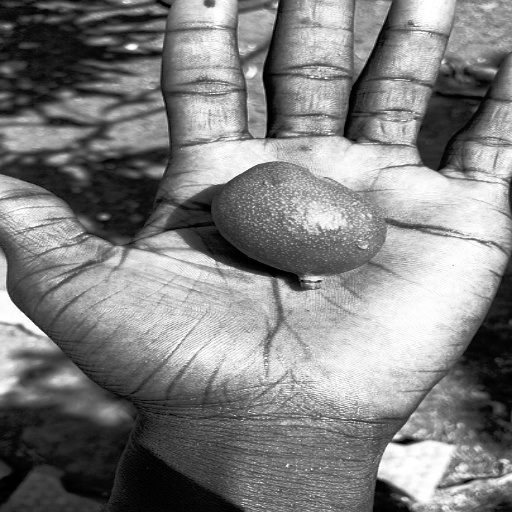
\includegraphics[height=2.5in]{images/log_raw}
        \caption{$I_1$}
    \end{subfigure}%
    ~ 
    \begin{subfigure}[t]{0.5\textwidth}
        \centering
        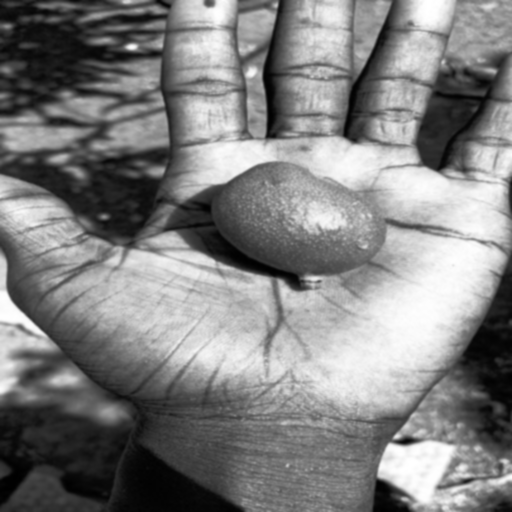
\includegraphics[height=2.5in]{images/log_g}
        \caption{$LPF(I_1)$}
        \label{fig:log_g}
    \end{subfigure}
    ~
    \vskip\baselineskip
    \begin{subfigure}[t]{0.5\textwidth}
        \centering
        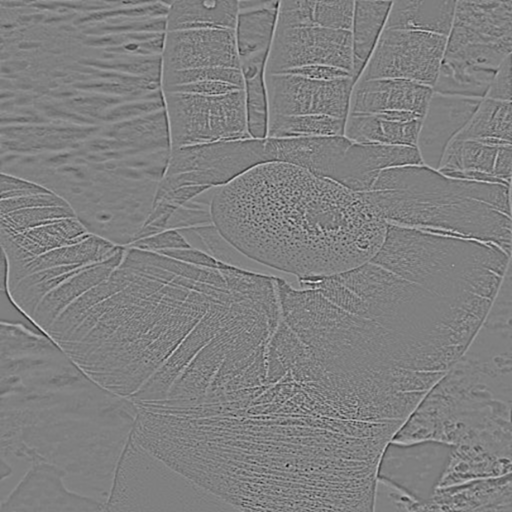
\includegraphics[height=2.5in]{images/log_log}
        \caption{$LoG(I_1)$}
        \label{fig:log_log}
    \end{subfigure}%
    ~
    \begin{subfigure}[t]{0.5\textwidth}
        \centering
        %TODO missing edge map
        %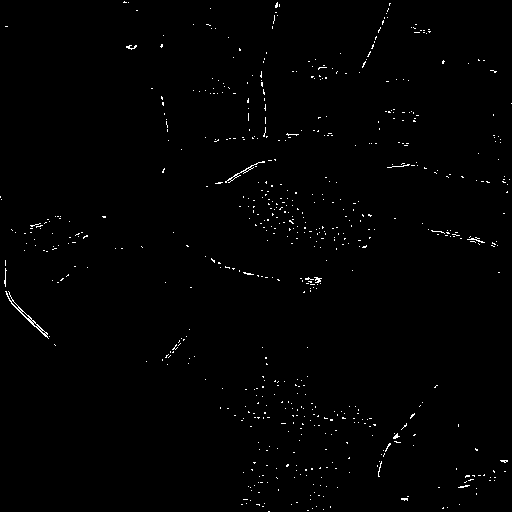
\includegraphics[height=2.5in]{images/log_edge}
        \caption{Edge map}
    \end{subfigure}
    \caption{LoG}
\end{figure}
Both \autoref{fig:log_g} and \autoref{fig:log_log} uses kernel size of 5 and $\sigma=1$. \autoref{fig:log_log} is ranged from $\lbrack -1, 1 \rbrack$. 

\paragraph*{Difference of Gaussians} is a feature enhancement method that involves the subtraction of one blurred version of an original image from another less blurred version of the original. 
In other word, first-order derivative of the Gaussian blurred image.

\begin{figure}[H]
    \centering
    \begin{subfigure}[t]{0.3\textwidth}
        \centering
        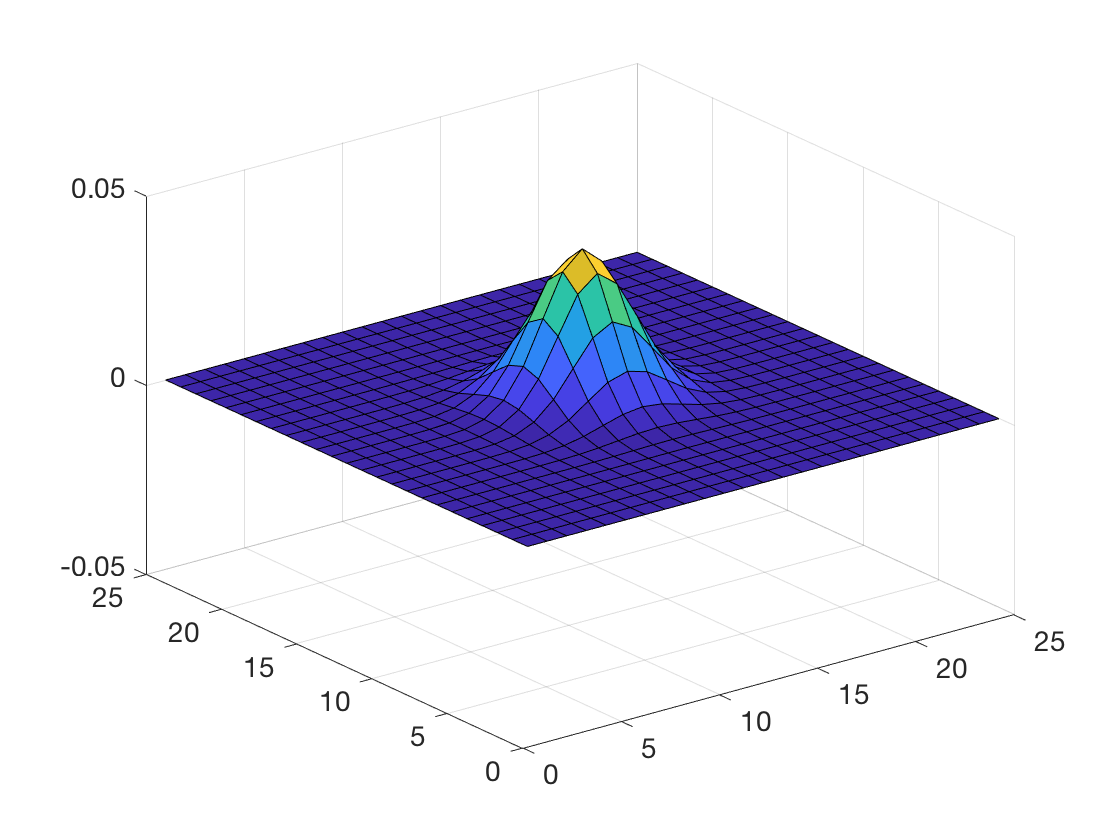
\includegraphics[height=2in]{images/dog_s2}
        \caption{$K_1$, $\sigma=2$}
    \end{subfigure}%
    ~ 
    \begin{subfigure}[t]{0.3\textwidth}
        \centering
        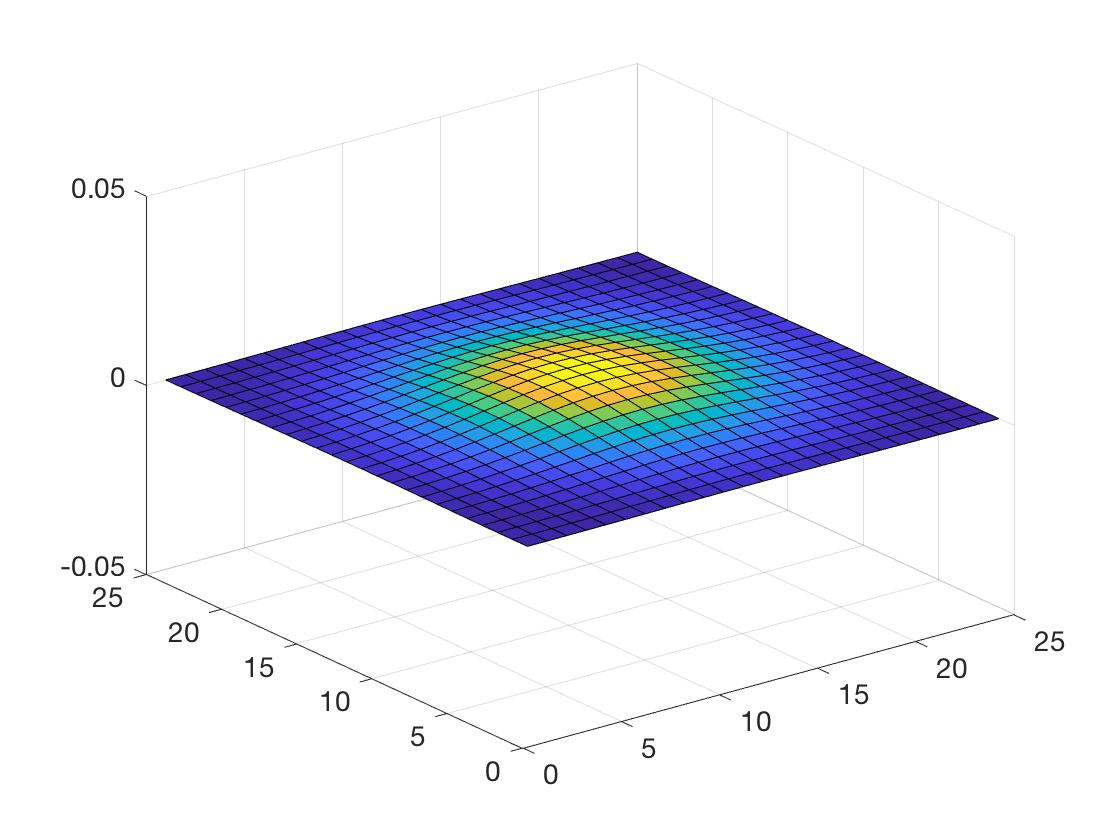
\includegraphics[height=2in]{images/dog_s5}
        \caption{$K_2$, $\sigma=5$}
    \end{subfigure}%
    ~
    \begin{subfigure}[t]{0.3\textwidth}
        \centering
        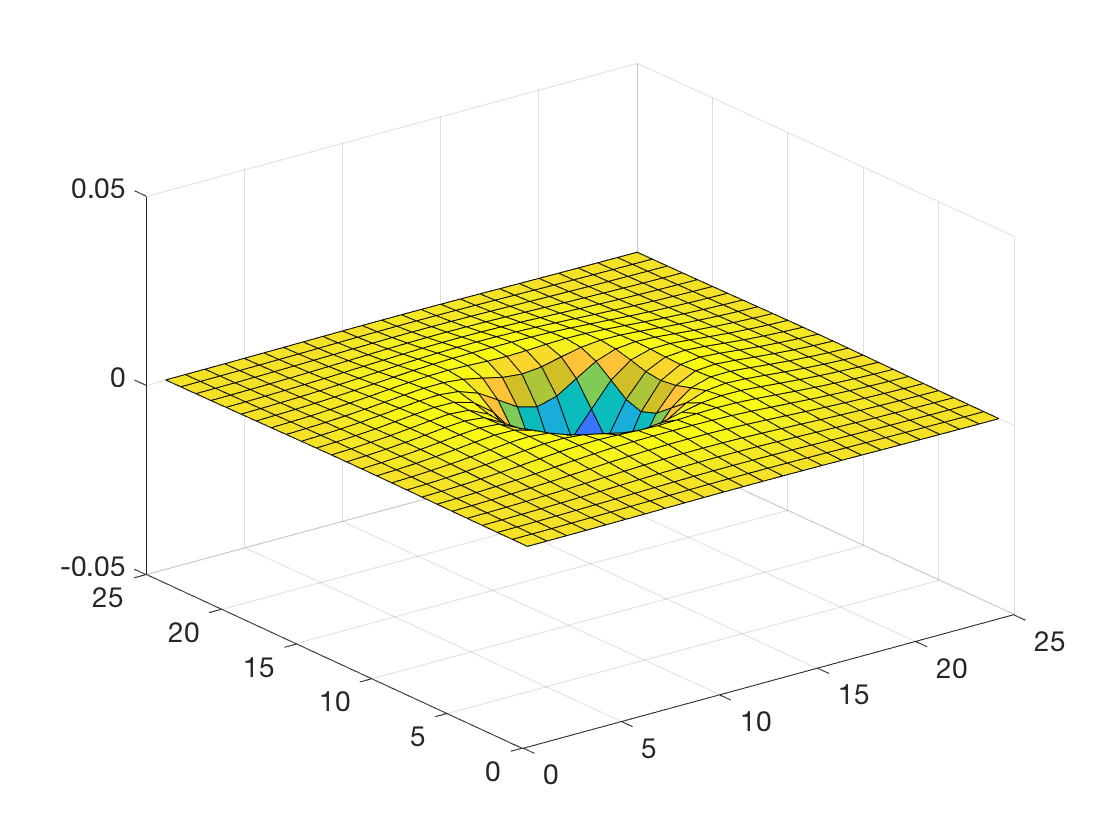
\includegraphics[height=2in]{images/dog_kernel}
        \caption{$K = K_2-K_1$}
    \end{subfigure}
    \caption{LoG}
    \label{fig:dog_kernel}
\end{figure}

\autoref{fig:dog_kernel} is the kernel used in this section, which is the result of subtracting Gaussian kernel of $\sigma = 5$ and $\sigma=2$.

\begin{figure}[H]
    \centering
    \begin{subfigure}[t]{0.5\textwidth}
        \centering
        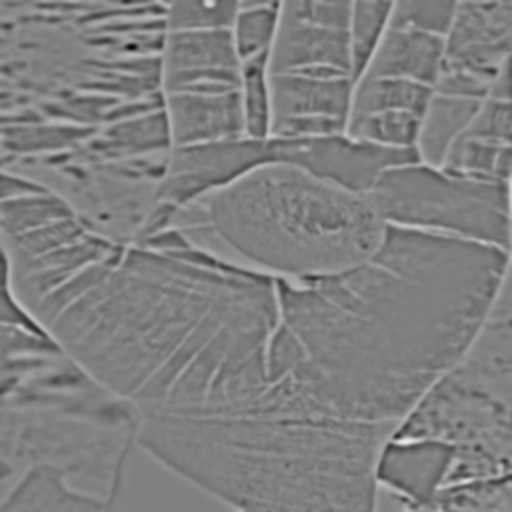
\includegraphics[height=2.5in]{images/dog_grad}
        \caption{DoG}
    \end{subfigure}%
    ~
    \begin{subfigure}[t]{0.5\textwidth}
        \centering
        %TODO edge map
        %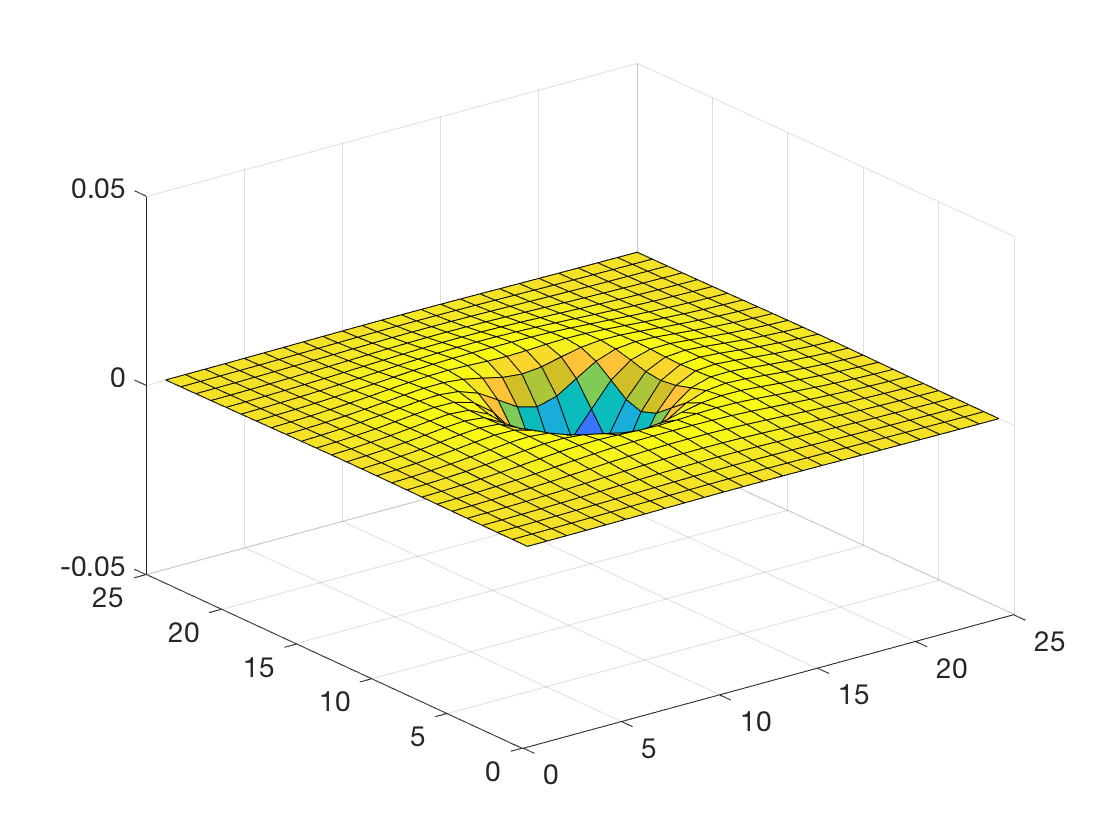
\includegraphics[height=2.5in]{images/dog_kernel}
        \caption{Edge map}
    \end{subfigure}
    \caption{LoG}
    \label{fig:dog}
\end{figure}

\subsection*{Canny edge detection}
\paragraph*{Step 1: Noise reduction}

\paragraph*{Step 2: Compute gradient magnitude and orientation}

\paragraph*{Step 3: Non-maximal suppression}

\paragraph*{Step 4: Hysteretic thresholding}

\paragraph*{Step 5: Connected component labeling}

\subsection*{Edges of noisy image}

\section*{Problem 2}
\subsection*{Edge crisping}
Basic operation is based on the unsharp filter
\begin{equation}
	C(x, y) = I_3(x, y) - K_n(\sigma) \ast I_3(x, y)
\end{equation}

\noindent
while $n$ is the kernel size and $\sigma$ is the standard deviation of the Gaussian function.
\autoref{fig:crisp_demo} demonstrates the generic effect of an unsharp filter.
\begin{figure}[H]
    \centering
    \begin{subfigure}[t]{0.3\textwidth}
        \centering
        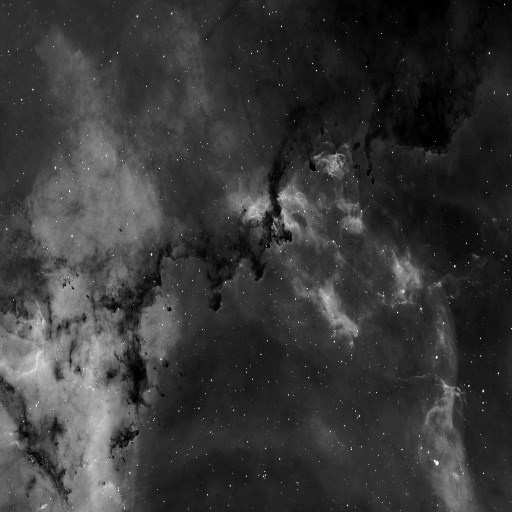
\includegraphics[height=2in]{images/crisp_raw}
        \caption{$I_3$}
    \end{subfigure}%
    ~ 
    \begin{subfigure}[t]{0.3\textwidth}
        \centering
        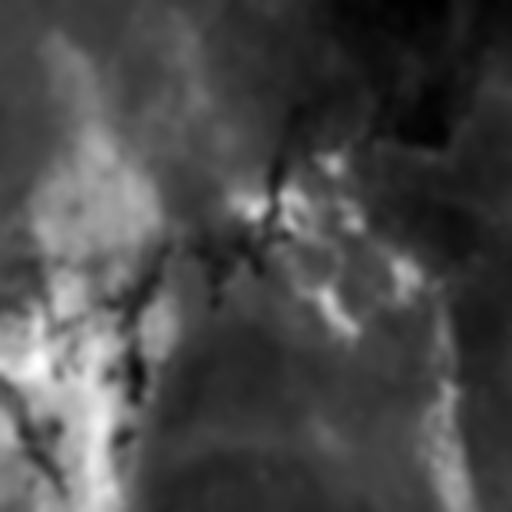
\includegraphics[height=2in]{images/crisp_smooth}
        \caption{$K \ast I_3$}
    \end{subfigure}%
    ~
    \begin{subfigure}[t]{0.3\textwidth}
        \centering
        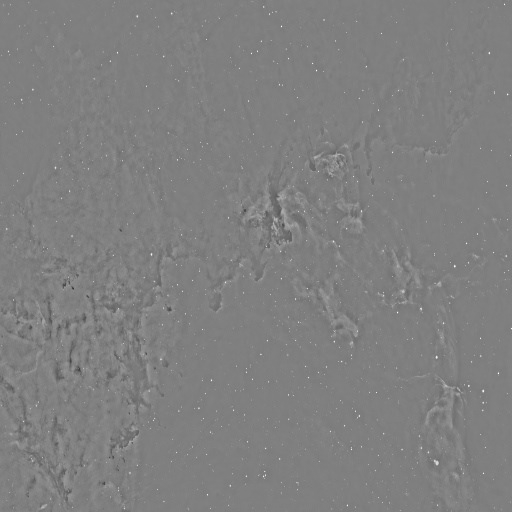
\includegraphics[height=2in]{images/crisp_crisp}
        \caption{$C$}
    \end{subfigure}
    \caption{LoG}
    \label{fig:crisp_demo}
\end{figure}
where $n$ is 15 and $\sigma$ is 5. One can easily distinguish the edge of the Milky Way and high visibility stars.

\begin{figure}[H]
    \centering
    \begin{subfigure}[t]{0.3\textwidth}
        \centering
        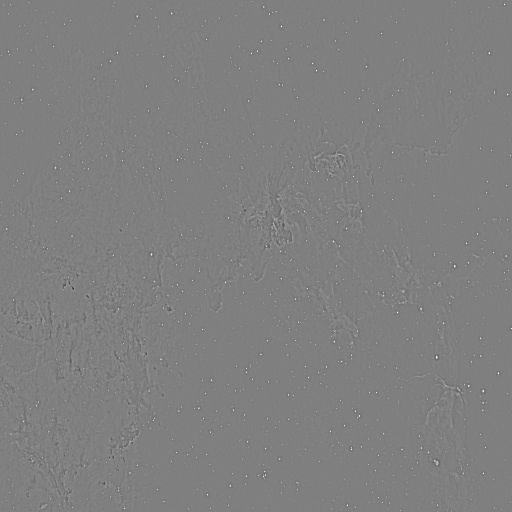
\includegraphics[height=2in]{images/crisp_n5s5}
        \caption{$n=5, \sigma=5$}
    \end{subfigure}%
    ~ 
    \begin{subfigure}[t]{0.3\textwidth}
        \centering
        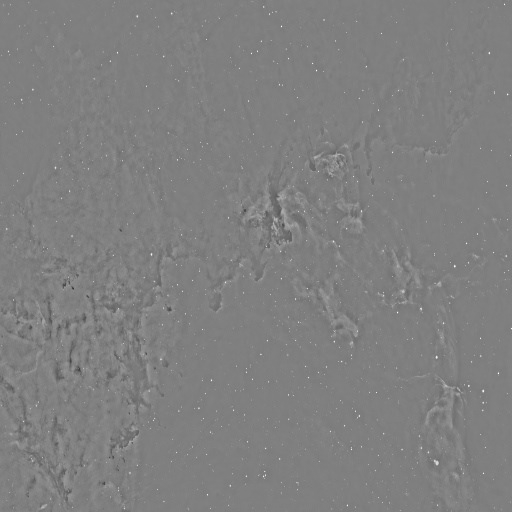
\includegraphics[height=2in]{images/crisp_n15s5}
        \caption{$n=15, \sigma=5$}
    \end{subfigure}%
    ~
    \begin{subfigure}[t]{0.3\textwidth}
        \centering
        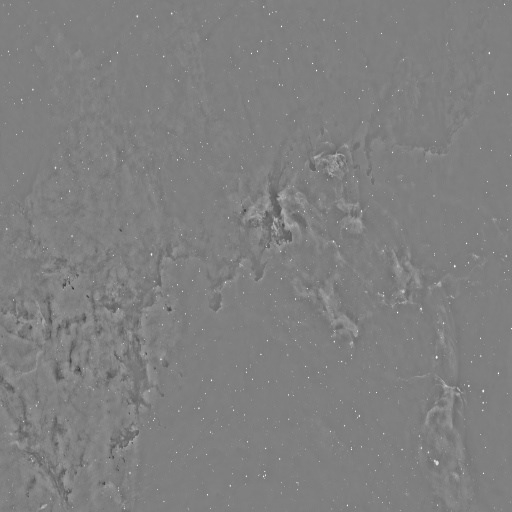
\includegraphics[height=2in]{images/crisp_n25s5}
        \caption{$n=25, \sigma=5$}
    \end{subfigure}
    ~
    \vskip\baselineskip
    \begin{subfigure}[t]{0.3\textwidth}
        \centering
        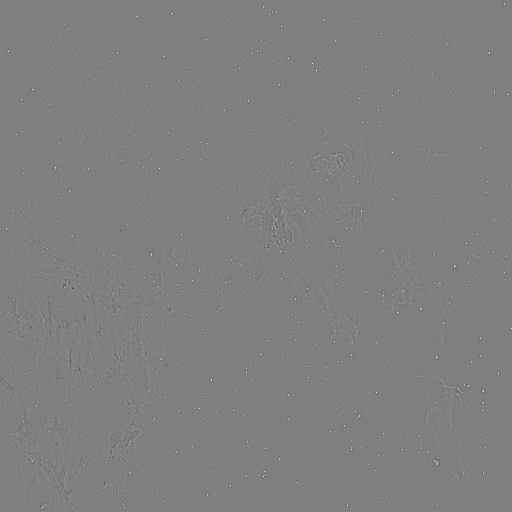
\includegraphics[height=2in]{images/crisp_n15s1}
        \caption{$n=15, \sigma=1$}
    \end{subfigure}%
    ~ 
    \begin{subfigure}[t]{0.3\textwidth}
        \centering
        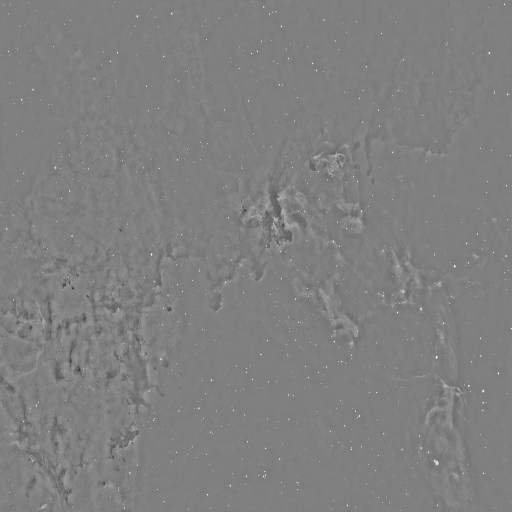
\includegraphics[height=2in]{images/crisp_n15s10}
        \caption{$n=15, \sigma=10$}
    \end{subfigure}%
    ~
    \begin{subfigure}[t]{0.3\textwidth}
        \centering
        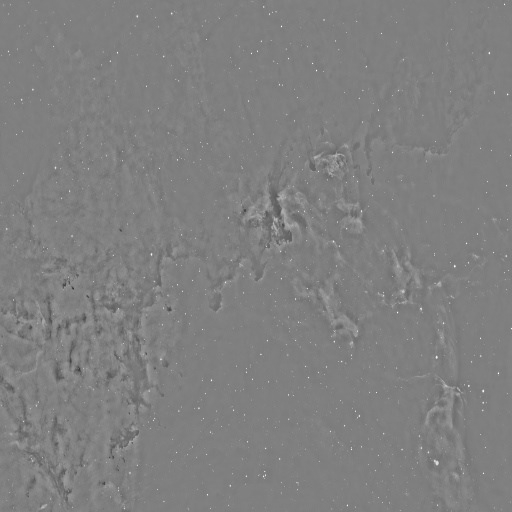
\includegraphics[height=2in]{images/crisp_n15s100}
        \caption{$n=15, \sigma=100$}
    \end{subfigure}%
    \caption{LoG}
    \label{fig:crisp_tune}
\end{figure}

While both increasing the kernel size and $\sigma$ enhance the result, increasing the kernel size while locking the $\sigma$ (first row in \autoref{fig:crisp_tune}) keeps the impulse noises indicates by the stars, which is reasonable due to the fact that out-skirt of the subtracted kernel is mostly zero, which is effectively a smaller blur kernel.

The second row in \autoref{fig:crisp_tune} increase the $\sigma$ while keep the kernel size at $n=5$, gradually increase the weighting of the surrounding pixels, hence the signals of stars gradually diminished (lower left region). 

When taking into consideration greater variety of the edge differences, aka, increase $n$, edge difference is more profound, due to considering less localized variations.
Increasing the $\sigma$ increases the differences per variation in pixel intensity, hence the features has greater contrast when comparing results between $n=15$ and $\sigma=5, 10$.

\subsection*{Warping}

\section*{Bonus}

\end{document}
              